%; whizzy paragraph -pdf xpdf -latex ./whizzypdfptex.sh
%; whizzy-paragraph "^\\\\begin{frame}"
% latex beamer presentation.
% platex, latex-beamer でコンパイルすることを想定。 

%     Tokyo Debian Meeting resources
%     Copyright (C) 2009 Junichi Uekawa
%     Copyright (C) 2010 Nobuhiro Iwamatsu

%     This program is free software; you can redistribute it and/or modify
%     it under the terms of the GNU General Public License as published by
%     the Free Software Foundation; either version 2 of the License, or
%     (at your option) any later version.

%     This program is distributed in the hope that it will be useful,
%     but WITHOUT ANY WARRANTY; without even the implied warranty of
%     MERCHANTABILITY or FITNESS FOR A PARTICULAR PURPOSE.  See the
%     GNU General Public License for more details.

%     You should have received a copy of the GNU General Public License
%     along with this program; if not, write to the Free Software
%     Foundation, Inc., 51 Franklin St, Fifth Floor, Boston, MA  02110-1301 USA

\documentclass[cjk,dvipdfmx,12pt]{beamer}
\usetheme{Tokyo}
\usepackage{monthlypresentation}
%  preview (shell-command (concat "evince " (replace-regexp-in-string "tex$" "pdf"(buffer-file-name)) "&"))
%  presentation (shell-command (concat "xpdf -fullscreen " (replace-regexp-in-string "tex$" "pdf"(buffer-file-name)) "&"))
%  presentation (shell-command (concat "evince " (replace-regexp-in-string "tex$" "pdf"(buffer-file-name)) "&"))

%http://www.naney.org/diki/dk/hyperref.html
%日本語EUC系環境の時
\AtBeginDvi{\special{pdf:tounicode EUC-UCS2}}
%シフトJIS系環境の時
%\AtBeginDvi{\special{pdf:tounicode 90ms-RKSJ-UCS2}}

\title{upstart 再入門}
\subtitle{}
\author{前田 耕平 mkouhei@debian.or.jp\\IRC nick: mkouhei}
\date{2010年4月17日}
\logo{
\includegraphics[width=8cm]{image200607/openlogo-light.eps}}

\begin{document}

\frame{\titlepage{}}

\begin{frame}
 \frametitle{深入りしようとしたのだが…。}

  \begin{itemize}
   \item 仕組みの深入りを試みたのだが…。
   \item 年度変わってプライベートの余力がなくて挫折。
   \item 2月とまったく同じのもどうかと。
  \end{itemize}
 そこでupstartの起動を bootchart で見てみた。
\end{frame}


\section{}
\begin{frame}
 \frametitle{事前準備}
 用意する インストールイメージ、パッケージ、
 \begin{itemize}
  \item debian-testing-amd64-businesscard.iso
  \item qemu-kvm パッケージ
  \item qcow2 フォーマットのディスクイメージ
  \item bootchart パッケージ
 \end{itemize}

 KVM/QEMU ゲストに sysvinit と upstart の2種類を用意
 \begin{itemize}
  \item Debian GNU/Linux Sid の最小構成をインストール
  \item インストール後、ディスクイメージからコピー作成
  \item コピー後、upstart パッケージをインストール
 \end{itemize}
 \end{frame}

\begin{frame}[containsverbatim]{upstart のインストール}
\begin{commandline}
$ sudo apt-get install upstart
(snip)
重大な問題を引き起こす可能性のあることをしようとしています。
続行するには、'Yes, do as I say!' というフレーズをタイプしてください。
 ?] Yes, do as I say!
\end{commandline}
 2月のときとは違い、今回は upstart をインストールしても問題なし。
 \footnote{lxc ではなく KVM/QEMU だから、なのか否かは未検証。}

\end{frame}

\begin{frame}{2月のおさらい : upstart の特徴}
サービス開始・停止はイベント通信に基づくこと。

起動させるプロセスを並行処理できることがメリット。

他の特徴は、
\begin{itemize}
 \item タスクやサービスの起動・停止でイベントが発生
 \item イベントはシステム上の他のプロセスから受け取る
 \item サービスが予期せず突然終了しても再起動する
 \item デーモンの監視と再起動は親プロセスから分離
 \item D-Bus を通じて init デーモンと通信
\end{itemize}

 プロセスを並行処理させることで処理速度を向上させるので、プロセスが多い
 ほど、効果は高いはず。
\end{frame}

\begin{frame}{起動速度を比べてみる}
 用意した環境は以下のとおり。

\begin{table}
\begin{tabular}[h]{|c|c|c|c|c|}\hline
initの種類 & 最小構成\footnote{bootchart はインストール} & CouchDB\footnote{最小構成に couchdb をインストール} & LAMP \footnote{CouchDB の構成に apache2,rails, mysql-server をインストール} & GNOME \footnote{最小構成に xserver-xorg, gnome をインストール} \\
\hline\hline
sysvinit & & & & \\
\hline
upstart & & & & \\
\hline
\end{tabular}
\end{table}
\end{frame}

\emtext{bootchart の結果}

\begin{frame}{最小構成}
\begin{minipage}[t]{0.48\hsize}
sysvinit
\begin{figure}[h]
\begin{center}
\includegraphics[width=1.0\hsize]{image201004/upstart/sysvinit-bootchart.eps}
\end{center}
\end{figure}
\end{minipage}
\begin{minipage}[t]{0.48\hsize}
upstart
\begin{figure}[h]
\begin{center}
\includegraphics[width=1.0\hsize]{image201004/upstart/upstart-bootchart.eps}
\end{center}
\end{figure}
\end{minipage}
\end{frame}

\begin{frame}{CouchDB}
\begin{minipage}[t]{0.48\hsize}
sysvinit
\begin{figure}[h]
\begin{center}
\includegraphics[width=1.0\hsize]{image201004/upstart/sysvinit-couchdb-bootchart.eps}
\end{center}
\end{figure}
\end{minipage}
\begin{minipage}[t]{0.48\hsize}
upstart
\begin{figure}[h]
\begin{center}
\includegraphics[width=1.0\hsize]{image201004/upstart/upstart-couchdb-bootchart.eps}
\end{center}
\end{figure}
\end{minipage}
\end{frame}
\begin{frame}{LAMP}
\begin{minipage}[t]{0.48\hsize}
sysvinit
\begin{figure}[h]
\begin{center}
\includegraphics[width=1.0\hsize]{image201004/upstart/sysvinit-lamp-bootchart.eps}
\end{center}
\end{figure}
\end{minipage}
\begin{minipage}[t]{0.48\hsize}
upstart
\begin{figure}[h]
\begin{center}
\includegraphics[width=1.0\hsize]{image201004/upstart/upstart-lamp-bootchart.eps}
\end{center}
\end{figure}
\end{minipage}
\end{frame}

\begin{frame}{GNOME}
\begin{minipage}[t]{0.48\hsize}
sysvinit
\begin{figure}[h]
\begin{center}
\includegraphics[width=1.0\hsize]{image201004/upstart/sysvinit-desktop-bootchart.eps}
\end{center}
\end{figure}
\end{minipage}
\begin{minipage}[t]{0.48\hsize}
upstart
\begin{figure}[h]
\begin{center}
\includegraphics[width=1.0\hsize]{image201004/upstart/upstart-desktop-bootchart.eps}
\end{center}
\end{figure}
\end{minipage}
\end{frame}

\begin{frame}{結果}

\begin{table}
\begin{tabular}{|c|c|c|c|c|}\hline
initの種類 & 最小構成\footnote{bootchart はインストール} &
 CouchDB\footnote{最小構成に couchdb をインストール} & LAMP
 \footnote{CouchDB の構成に apache2,rails, mysql-server をインストール} & GNOME
 \footnote{最小構成に xserver-xorg, gnome をインストール} \\
\hline\hline
sysvinit & 5 sec & 6 sec & 8 sec & 8 sec \\
\hline
upstart & 5 sec & 6 sec & 8 sec & 8 sec \\
\hline
\end{tabular}
\end{table}
起動時間にはまったく違いなし…。
\end{frame}

\begin{frame}{そういえば、忘れていた。}
 \begin{itemize}
  \item Debian の upstart は互換モードなので、sysvinit の動作を模倣して
	いるのだった。
  \item これでは比較にならん。
 \end{itemize}
\end{frame}

\begin{frame}{Ubuntu 9.10 を試してみた。}
\begin{minipage}[t]{0.48\hsize}
\begin{itemize}
 \item Ubuntu 9.10 ではネイティブモード
 \item Debian に比べると最小構成に余計なパッケージがあるみたい
 \item init の処理終了時で bootchart のログ収集を止めるわけでは
       ないようだが、実質的には25秒程度で起動が完了。
 \item でも起動プロセスが並行処理されていること Debian での結果を比べて
       も分かる。
\end{itemize}
\end{minipage}
\begin{minipage}[t]{0.48\hsize}
\begin{figure}[h]
\begin{center}
\includegraphics[width=1.0\hsize]{image201004/upstart/ubuntu-karmic-20100417-3.eps}
\end{center}
\end{figure}
\end{minipage}
\end{frame}

\begin{frame}{まとめ}
\begin{itemize}
 \item ネイティブモードじゃないと upstart は本来のメリットが活かせない感
       じ。
 \item とはいえ、いきなりネイティブモードの upstart に切り替えるのはリス
       クあるので、一時的に互換モードを使うのは止むを得ないのかもしれな
       い。
 \item でも、Squeeze でずっと互換モードなのもどうかと。SqueezeAndAHalf
       リリース時にネイティブモードに切り替えられるとうれしいかも。
\end{itemize}

\end{frame}

\end{document}

;;; Local Variables: ***
;;; outline-regexp: "\\([ 	]*\\\\\\(documentstyle\\|documentclass\\|emtext\\|section\\|begin{frame}\\)\\*?[ 	]*[[{]\\|[]+\\)" ***
;;; End: ***
